% Figure 1 - experiment 01, Bitcoin Core wallet case study.
% Generated by figures/plot_crossover.py from data/wallet_sweep_20rep.csv.
% Full text width; for a single column use [width=\columnwidth] and figure/.
\begin{figure*}[t]
  \centering
  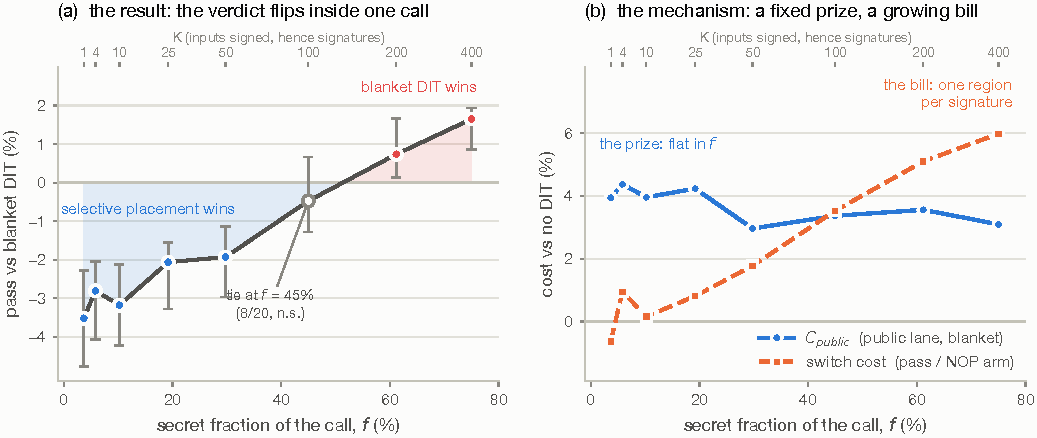
\includegraphics[width=\textwidth]{figures/crossover.pdf}
  \caption{%
    \textbf{The secret-fraction crossover, inside one unmodified Bitcoin Core
    wallet call.}
    \texttt{WalletCreateTxUsePresetInputsAndCoinSelection} on Apple M5, 20
    paired repetitions per cell with arm order rotated every repetition.
    The knob is $K$, the number of inputs the transaction spends and hence the
    number of \texttt{CKey::Sign} calls; it moves only the ratio between a real
    public lane (coin selection) and a real secret lane (ECDSA signing), and
    $f$ is the resulting secret fraction \emph{measured} by re-running with
    signing disabled.
    \textbf{(a)}~Selective \texttt{PSTATE.DIT} placement against blanket DIT.
    Below zero the pass is faster. Filled markers are resolved by an exact
    two-sided sign test at $p<0.05$; the hollow marker at $f = 45\%$ is not.
    Bars are distribution-free $95.9\%$ confidence intervals for the median
    (order statistics 6--15 of 20), so they agree with the sign test by
    construction.
    \textbf{(b)}~Why. The prize---what blanket DIT costs on the public lane
    alone---is flat in $f$, because blanket DIT protects everything either way.
    The pass's own cost grows with the secret lane it protects, and their
    crossing in~(b) is the zero crossing in~(a).
    The growing curve is \texttt{pass/passnop}. It is \emph{not} the switch
    cost: the NOP arm emits \texttt{HINT~\#0} in place of every inserted
    \texttt{MSR~DIT}, so \texttt{PSTATE.DIT} is never set and that arm loses
    the protection as well as the switch. The curve is the switch \emph{plus}
    DIT dwell over the protected regions. Running one binary under two
    \textsc{msr dit} implementations in gem5 isolates serialisation at
    $+1.21\%$ at $K=400$, against the $+5.98\%$ this curve reports.
    Panel~(a) is unaffected: \texttt{pass} and \texttt{blanket} both protect
    the secret lane, so the dwell term is present in both and cancels.
    Numbers are identical to Table~\ref{tab:crossover}; the plotting script
    asserts this.%
  }
  \label{fig:crossover}
\end{figure*}
